\section{Getting Started}

This section will outline how to quickly set up and use the program.

It is important to note before we begin, that every game
\textbf{MUST} have a unique
name. If there are two games with the same name, then find some way
to denote them differently. For example, entering the games manually
as "Game (Type A)" and the second game as "Game (Type B)".

\subsection{Adding}

To begin, we need some data! There are several options for adding
data to your LoGL. By clicking the "Add" button, you can see the
entire list of available options. This guide will go through them in
order from top to bottom.

\subsubsection{Game Search}

\begin{figure}[htb]
	\centering
	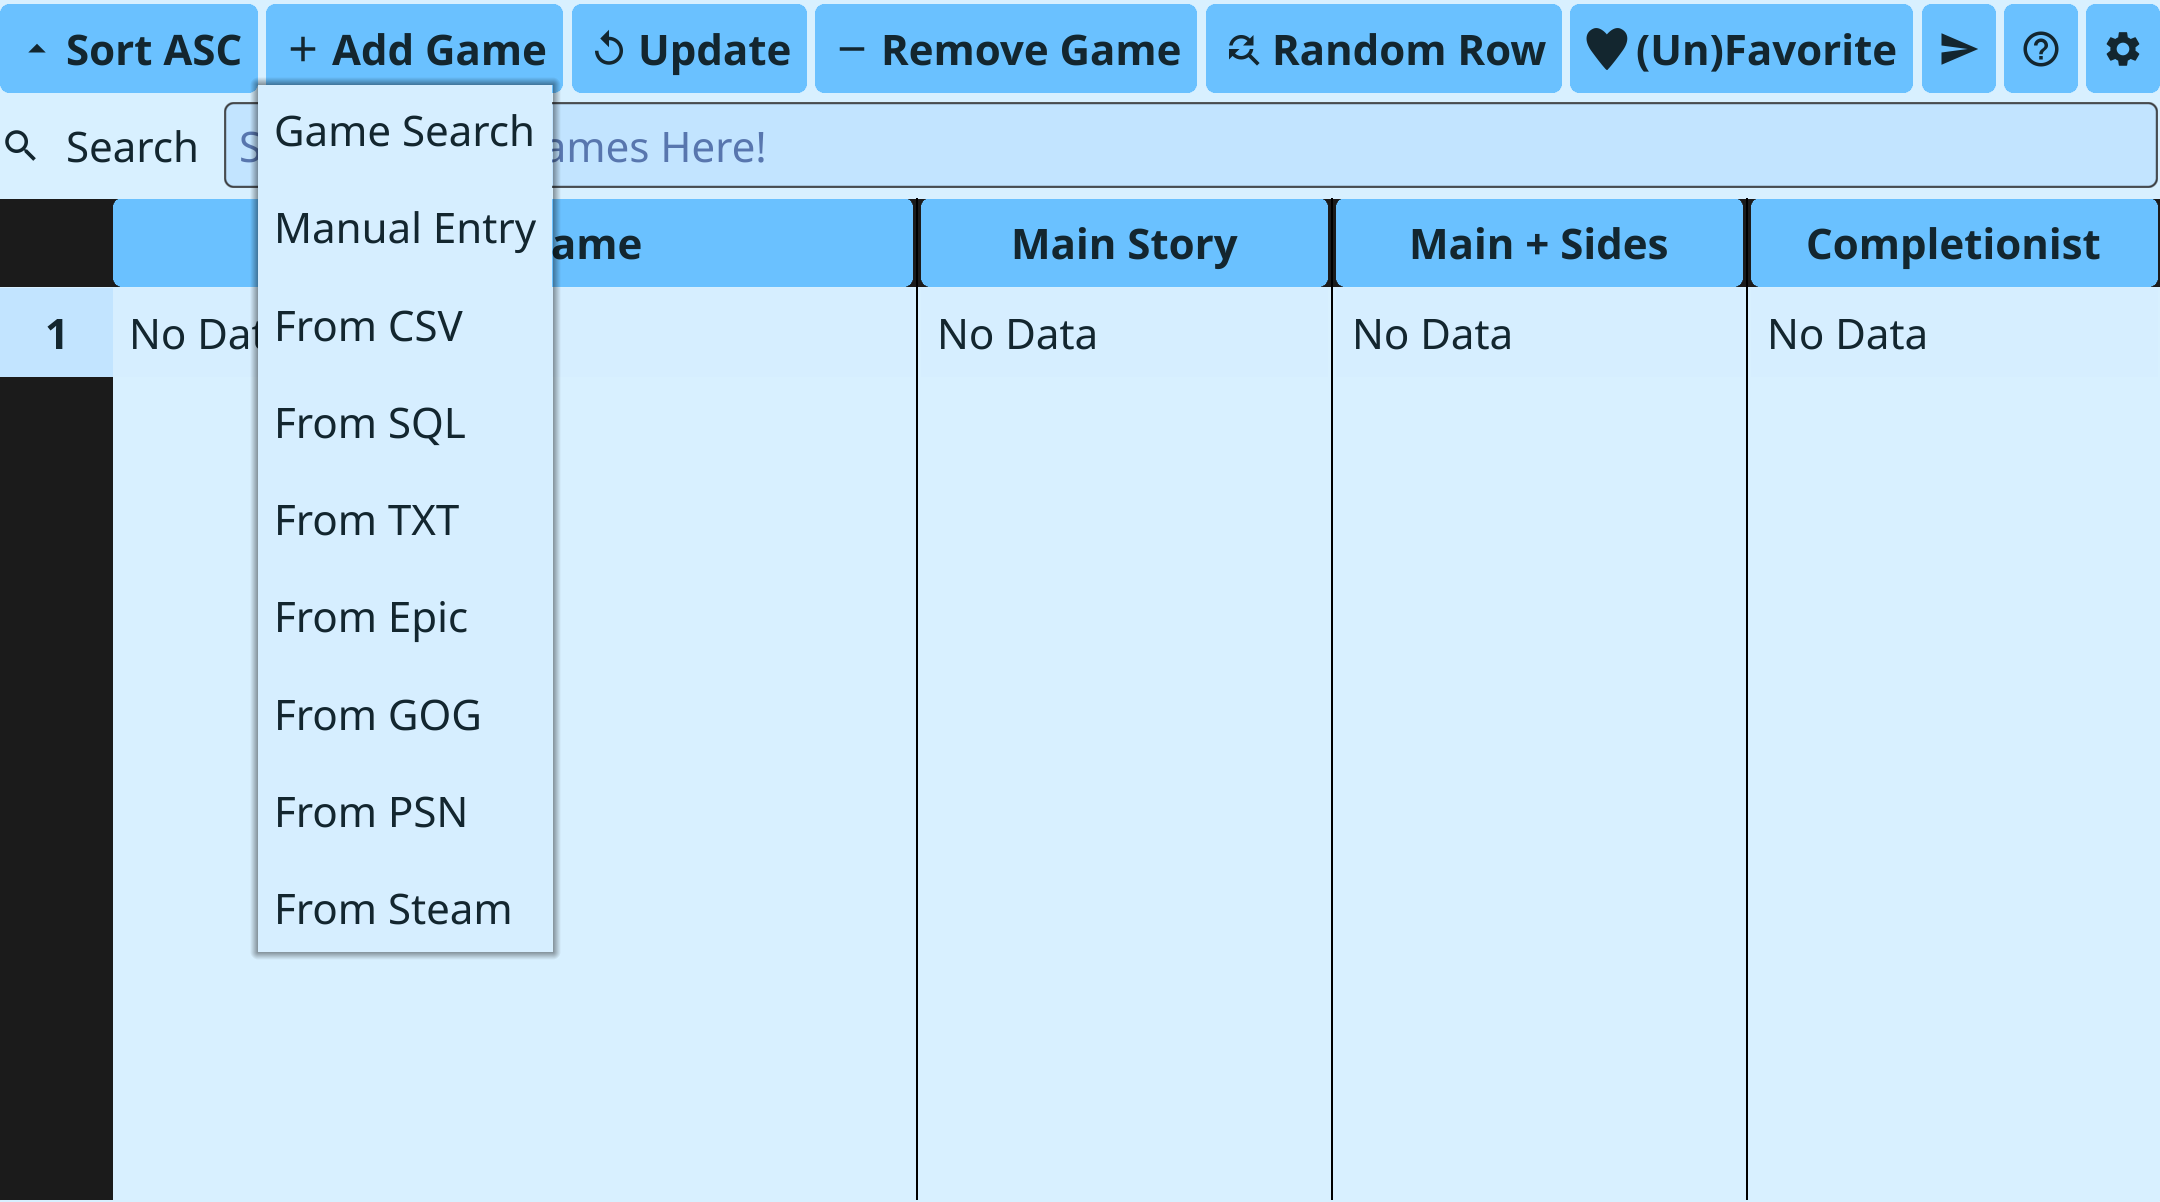
\includegraphics[width=14cm]{./Images/AddOpts.png}
	\caption{List of options to add game data}
	\label{fig:AddOpts}
\end{figure}

If you have a single game that you want to search, then use the "Game
Search" option. This will open a text box for you to search the game.
Enter the specified game name. In the example below, I use "Metroid"
to demonstrate the program searching for the NES classic.

% TODO: Insert image of text box with metroid
% TODO: Insert image of database before and after entering metroid

You have now added your first game to your LoGL!

Perhaps the program didn't find the game you were looking for. In
this case, the first option is to try again. Sometimes the program
doesn't get it quite right. In this case, make sure to properly spell the name.
If that doesn't work, then not to worry! There are other ways to import data.

\subsubsection{Manual Entry}

Instead of having the program find the data on the internet, you can
enter the data yourself! The only required information is the: Name,
Main Story, Main + Sides, and Completionist values. The URLs for the
search sources are unnecessary, but make the updating process
(discussed later in section \ref{subsec:Updating}) work properly.

Please ensure that you enter the data properly for the time entries.
They must be in decimal format (e.g. 15.6 meaning 15.6 Hours or 15
hours and 36 minutes).

The URLs are to be copied as is for the game, should you wish to provide them.

% TODO: Image of menu for manual entry with proper formatting vs
% improper formatting

%TODO: Show image of database now with the game search and manual
% entry - Metroid (3DS Virtual Console)

\subsubsection{Importing from different Files}

The next three options allow you to import data from different file
types: CSV, SQL, and TXT. Of the three, SQL is destructive, meaning
that it will \textbf{COMPLETELY DELETE ALL DATA IN THE DATABASE}
before it adds the new data. Importing from either CSV or TXT is
non-destructive, meaning that it can only add new data to the
database. Any duplicate entries found are discarded and not utilized.

Select the desired file to import based on the file type. In the
following example, I will use a TXT file. After seeing the list of
add options, select the "From TXT" option. This will open a menu
showing you your file system. Locate the file you wish to import from
and click "Open". The data will be promptly imported.

% TODO: image of importing from TXT file
% 1. highlight form txt
% 2. show filesystem with the locaiton of the file to import from
% 3. Show the changes to the database

TXT files are the only ones that require special formatting not
handled by this program.
TXT files must have each line be the name of a single game. Once
again, spelling is of great importance in order for the program to
add the data properly.

% TODO: image of good vs bad TXT file.
% highlight differences in clear colors. red is bad, green is good.
% checks and x's.

\subsubsection{Importing from Integrations}

This section is the most involved and technical.

As of Version 1.0.0, there are 4 Integrations that are supported.
They each require user input in order to work properly, with some
requiring you to enter the cookie for the integration to work. I will
walk you through this process from start to finish with images at
each step for clarity.

If you feel uncomfortable inputting your cookie information, or using
the developer web-tools in your browser, then feel free to skip this section.

step 0a: getting dev-tools unlocked for your browser:
showcase in chrome and firefox. these two are the big ones and
generally are the flagship styles that other browsers use as a base.
It won't cover all browsers, but will cover a vast majority of them.

step 0b: pick an integration.

% TODO: walk through process for each integration

\paragraph{Epic}

% TODO: add the images for each step
\begin{enumerate}
	\item In your preferred browser, sign into epic games by going to
		this link: \href{}{link here.}
	\item Click "Account"
	\item Click "Apps \& Accounts".
	\item Open developer tools in your browser.
	\item Go to the network tab in developer tools.
	\item Click on the "Apps" tab in the browser page.
	\item Find the "authorized-apps" entry from the list in developer tools.
	\item Open the page.
	\item Copy the contents of the page and input into the program.
\end{enumerate}

\paragraph{GOG}

% TODO: add the images for each step
\begin{enumerate}
	\item In your preferred browser, sign into GOG by going to
		this link:

		\href{https://embed.gog.com/account/getFilteredProducts?mediaType=1&page=1}{https://embed.gog.com/account/getFilteredProducts?mediaType=1\&page=1}
	\item Open developer tools in your browser.
	\item Depending on your browser, you will need to find the location
		of the data. In chrome, it is called "Application", while in
		Firefox it is called "Storage".
	\item View cookies for the website (GOG).
	\item Find the "gog\_us" cookie.
	\item Copy the contents of the cookie and input into the program.
\end{enumerate}

\paragraph{PSN}

There is a prerequisite to use this integration. That is the Chrome
browser to be installed. Assuming it is installed, and you want to
continue to use this integration, follow the below steps to set it up.

This only works for games that have...

% TODO: add the images for each step
\begin{enumerate}
	\item First you must ensure that the account has a publicly viewable
		set of data. I will describe the sequence of steps to set that up now.
		\begin{enumerate}
			\item yuh
		\end{enumerate}
	\item Enter the psn profile name into the program.
\end{enumerate}

\paragraph{Steam}

% TODO: add the images for each step
\begin{enumerate}
	\item Login from any browser at the following link:

		\href{https://steamcommunity.com/id/PROFILE/games/?tab-all}{https://steamcommunity.com/id/PROFILE/games/?tab-all}.
	\item Open developer tools.
	\item Go to application on chrome, or storage on firefox
	\item view cookies for webpage (steam)
	\item locate the "sessionid" cookie
	\item copy the contents and paste into the program
\end{enumerate}

\subsection{Updating}
\label{subsec:Updating}

Should you want to update the data to be more recent, then all you
have to do is click on the row with the desired game, and click the
update button. This then updates the given game with the new data
found from the internet. This always overwrites the previous data.
Sometimes the new data that is grabbed is the same as the old data,
so there is no change.

% TODO: image of process:
% 1. select game to update
% 2. press update button
% 3. see values change

\subsection{Removing}

If you want to delete a particular game from the library, then click
on the row with the desired game, then click the remove game button.
This will remove the game data.

% TODO: image of process:
% 1. select game to delete
% 2. press delete
% 3. show database has changed

\subsection{Searching within the database}

If you want to search for all games matching a given text (e.g.
"Met" in hopes of finding Metroid), then the view will automatically
update to show all found options. It also shows partial matches too,
including within words (e.g. "Met" would also return Metro Exodus,
Metal Gear Solid, and Symmetry).

% TODO: image of database without searched text
% then show final result after typing "Met" to show all options:
% Metroid, Metroid (3DS Virtual Console), Metro Exodus, Metal Gear
% Solid, and Symmetry

\subsection{Changing the View}

Not only can you modify the contents of the library, but you can also
change the view of it.
By clicking any of the columns of the table (Main Story, Main +
Sides, and Completionist) you can choose which way you want the data
to be sorted by. Furthermore, you can choose it to be sorted
ASCending or DESCending via the first button in the menu.

% TODO: Show how the database view changes when selecting different options

% TODO: image demonstrating how the sorts work:
% Game name
% Main
% MAin +
% Comp
% with a series of arrows indicating Ascending vs. Descending.
% Showcase different values like negatives, non-standard letters,
% and capitalization.

\subsection{Settings}

you can manage stuff here like:
deleting all the data in the database
updating all the games in the database
changing the search source
changing the text and icon size
or picking a theme.

you can create your own themes which is discussed in the advanced section.
